% Generado desde README.md. Editar libremente.

\section{3. Sistemas, componentes e integración}

\begin{landscape}
Cuatro sistemas se reparten el negocio: inventario (qué se vende y cuánto queda), pedidos (qué pasó con cada compra), clientes (quién compra) y pagos (el dinero). La regla de esta sección es que cada dato tenga un solo dueño, que es quien decide su estado oficial. La matriz dice qué hace cada sistema, de quién depende, con qué llave se lo llama y qué ocurre si falla; la secuencia de más abajo cuenta la compra de Javiera paso a paso.

\subsection{Matriz de sistemas}
Los cuatro sistemas mínimos del caso son microservicios privados, cada uno con su base y su usuario de Mongo. Cada uno decide el estado oficial de sus datos; los demás lo consultan por contrato.

\vspace{0.6em}
{\scriptsize
\setlength{\LTpre}{0pt}\setlength{\LTpost}{0pt}
\setlength{\tabcolsep}{3pt}\renewcommand{\arraystretch}{1.15}
\begin{longtable}{|>{\raggedright\arraybackslash}p{\dimexpr 0.0668\linewidth-2\tabcolsep\relax}|>{\raggedright\arraybackslash}p{\dimexpr 0.1465\linewidth-2\tabcolsep\relax}|>{\raggedright\arraybackslash}p{\dimexpr 0.1465\linewidth-2\tabcolsep\relax}|>{\raggedright\arraybackslash}p{\dimexpr 0.0540\linewidth-2\tabcolsep\relax}|>{\raggedright\arraybackslash}p{\dimexpr 0.1465\linewidth-2\tabcolsep\relax}|>{\raggedright\arraybackslash}p{\dimexpr 0.1465\linewidth-2\tabcolsep\relax}|>{\raggedright\arraybackslash}p{\dimexpr 0.1465\linewidth-2\tabcolsep\relax}|>{\raggedright\arraybackslash}p{\dimexpr 0.1465\linewidth-2\tabcolsep\relax}|}
\hline
\textbf{Sistema} & \textbf{Responsabilidad} & \textbf{Datos bajo su autoridad (estado oficial)} & \textbf{Servicios asociados} & \textbf{Dependencias} & \textbf{Contrato de integración} & \textbf{Credencial o identidad} & \textbf{Respuesta ante fallos} \\ \hline
\endfirsthead
\hline
\textbf{Sistema} & \textbf{Responsabilidad} & \textbf{Datos bajo su autoridad (estado oficial)} & \textbf{Servicios asociados} & \textbf{Dependencias} & \textbf{Contrato de integración} & \textbf{Credencial o identidad} & \textbf{Respuesta ante fallos} \\ \hline
\endhead
inventory (\texttt{inventario}) & Catálogo, precios, reglas de armado, cotización, stock y reservas & Producto, su precio y su disponibilidad; reservas (decide si hay unidades) & S01 a S06 & Ninguna: no llama a nadie & REST público (S01 a S06) y de integración: \texttt{POST /\allowbreak{}internos/\allowbreak{}cotizar}, \texttt{POST /\allowbreak{}internos/\allowbreak{}reservas}, \texttt{POST /\allowbreak{}internos/\allowbreak{}reservas/\allowbreak{}:\allowbreak{}pedido/\allowbreak{}liberar} & Recibe \texttt{X-\allowbreak{}Credencial-\allowbreak{}Interna} (\texttt{internos/\allowbreak{}inventario}); usuario de Mongo propio & Si no responde, pedidos no crea el pedido (\texttt{502/\allowbreak{}504}): nunca confirma sin cotizar. La reserva descuenta el stock ítem por ítem con la condición \texttt{stock >=\allowbreak{} cantidad} y, si uno no alcanza, devuelve lo ya descontado (\texttt{409 SIN\_\allowbreak{}STOCK}); es idempotente por pedido, se libera al anular y liberar dos veces devuelve el stock una sola vez \\ \hline
orders (\texttt{pedidos}) & Creación y ciclo de vida del pedido, venta, boleta, colas de cocina y despacho, reporte & Estado del pedido, venta y boleta (decide si un pedido está pagado, en preparación o entregado) & S15 a S26 & inventario (cotizar, reservar, liberar), clientes (ficha), pagos (devolución), ActiveMQ (publica) & REST público; interno \texttt{POST /\allowbreak{}internos/\allowbreak{}pedidos/\allowbreak{}:\allowbreak{}id/\allowbreak{}pago-\allowbreak{}confirmado}; eventos STOMP \texttt{/\allowbreak{}queue/\allowbreak{}correos} y \texttt{/\allowbreak{}queue/\allowbreak{}cocina} & Recibe \texttt{internos/\allowbreak{}pedidos}; usa las credenciales de inventario, clientes y pagos para llamarlos & Inventario o clientes caídos: \texttt{502/\allowbreak{}504}, no se crea nada. Falla de ActiveMQ: el pago se registra igual y el aviso queda en el log. Confirmar dos veces el mismo pago no hace nada la segunda vez \\ \hline
clients (\texttt{clientes}) & Registro, perfil y acceso autorizado a los datos del cliente & Ficha personal y si está activa (la cuenta y su verificación las decide Auth) & S07 a S14 & Auth Service (crear cuenta, cambiar estado, ver verificación) & REST público; interno \texttt{GET /\allowbreak{}internos/\allowbreak{}clientes/\allowbreak{}:\allowbreak{}id} (lo usa pedidos) & Recibe \texttt{internos/\allowbreak{}clientes}; ante Auth usa \texttt{internos/\allowbreak{}auth-\allowbreak{}clientes} (Basic, solo \texttt{/\allowbreak{}cuentas}) & Si Auth falla al registrar, se borra la ficha recién creada (compensación) y se responde el error. Si clientes no responde, pedidos responde \texttt{502/\allowbreak{}504} \\ \hline
payments (\texttt{pagos}) & Iniciar pagos, comprobar el resultado y relacionarse con el proveedor & Estado y monto del pago (el estado del \emph{pedido} lo decide pedidos) & S27 a S29 & pedidos (propiedad, monto y confirmación), pasarela (crear la transacción y devolver) & REST público; webhook firmado; interno \texttt{POST /\allowbreak{}internos/\allowbreak{}devoluciones} y \texttt{GET /\allowbreak{}internos/\allowbreak{}pagos} & Recibe \texttt{internos/\allowbreak{}pagos}; ante la pasarela usa \texttt{pasarela/\allowbreak{}comercio} (\texttt{api\_\allowbreak{}key}) y verifica \texttt{secreto\_\allowbreak{}firma} & Pasarela caída al iniciar: \texttt{502}. Si pedidos no responde al confirmar, se responde \texttt{502} y la pasarela reintenta (3 veces); la repetida reintenta solo el aviso a pedidos \\ \hline
\end{longtable}
}
\end{landscape}

\textbf{Quién autoriza el cambio de estado de un pago.} El aviso del proveedor se verifica en cuatro pasos: (1) firma HMAC-SHA256 del cuerpo exacto con el \texttt{secreto\_\allowbreak{}firma} que está en Vault; (2) el \texttt{token} y la orden corresponden a un pago registrado; (3) el monto coincide con el del pago (y pedidos vuelve a exigir que sea el total del pedido); (4) el cambio se aplica con una condición atómica (\texttt{estado:\allowbreak{} PENDIENTE} en el mismo \texttt{update}), de modo que una notificación repetida responde \texttt{repetido:\allowbreak{} true} sin registrar otra venta. Solo entonces pagos avisa a pedidos, y \textbf{pedidos es el único que cambia el estado del pedido a \texttt{PAGADO}}, emite la boleta y registra la venta. El frontend no decide nunca que un pedido está pagado: solo muestra lo que devuelve el servidor.


\textbf{orders e inventory.} Pedidos consulta a inventario, antes de aceptar el pedido, el precio y la disponibilidad de cada ítem (\texttt{cotizar}) y reserva las unidades (\texttt{reservas}). Si inventario no responde en 4~s, el pedido no se crea. Para no confirmar unidades que ya no existen, cada ítem se descuenta con una condición sobre el stock en la misma operación de actualización (\texttt{stock >=\allowbreak{} cantidad}), de modo que dos compras simultáneas no se llevan la misma unidad; si un ítem no alcanza, se devuelve lo ya descontado y el cliente recibe \texttt{SIN\_\allowbreak{}STOCK}.


\subsection{Estados del pedido y quién los cambia}

{\small
\setlength{\tabcolsep}{3pt}\renewcommand{\arraystretch}{1.15}
\begin{longtable}{|>{\raggedright\arraybackslash}p{\dimexpr 0.2178\linewidth-2\tabcolsep\relax}|>{\raggedright\arraybackslash}p{\dimexpr 0.2178\linewidth-2\tabcolsep\relax}|>{\raggedright\arraybackslash}p{\dimexpr 0.2251\linewidth-2\tabcolsep\relax}|>{\raggedright\arraybackslash}p{\dimexpr 0.3392\linewidth-2\tabcolsep\relax}|}
\hline
\textbf{Desde} & \textbf{Hacia} & \textbf{Operación (ID)} & \textbf{Quién} \\ \hline
\endfirsthead
\hline
\textbf{Desde} & \textbf{Hacia} & \textbf{Operación (ID)} & \textbf{Quién} \\ \hline
\endhead
(nuevo) & PENDIENTE\_\allowbreak{}PAGO & S15 & cliente \\ \hline
PENDIENTE\_\allowbreak{}PAGO & PAGADO & confirmación de pago (interna, desde S29) & pagos, con la credencial de pagos; el monto debe coincidir \\ \hline
PAGADO & EN\_\allowbreak{}PREPARACION & S20 & cocina, admin \\ \hline
EN\_\allowbreak{}PREPARACION & LISTO\_\allowbreak{}DESPACHO o LISTO\_\allowbreak{}RETIRO & S21 & cocina, admin \\ \hline
LISTO\_\allowbreak{}DESPACHO & EN\_\allowbreak{}DESPACHO & S22 & despacho, admin \\ \hline
EN\_\allowbreak{}DESPACHO o LISTO\_\allowbreak{}RETIRO & ENTREGADO & S23 & despacho, admin \\ \hline
PENDIENTE\_\allowbreak{}PAGO o PAGADO & ANULADO & S25 & cliente (suyo), admin \\ \hline
\end{longtable}
}

\subsection{Servicios propios y proveedores externos}

{\small
\setlength{\tabcolsep}{3pt}\renewcommand{\arraystretch}{1.15}
\begin{longtable}{|>{\raggedright\arraybackslash}p{\dimexpr 0.1840\linewidth-2\tabcolsep\relax}|>{\raggedright\arraybackslash}p{\dimexpr 0.2324\linewidth-2\tabcolsep\relax}|>{\raggedright\arraybackslash}p{\dimexpr 0.4128\linewidth-2\tabcolsep\relax}|>{\raggedright\arraybackslash}p{\dimexpr 0.1707\linewidth-2\tabcolsep\relax}|}
\hline
\textbf{Pieza} & \textbf{Propia o externa} & \textbf{Qué hace} & \textbf{Cómo se prueba} \\ \hline
\endfirsthead
\hline
\textbf{Pieza} & \textbf{Propia o externa} & \textbf{Qué hace} & \textbf{Cómo se prueba} \\ \hline
\endhead
Despacho & Propia (dentro de pedidos) & Cola, chofer y entrega; comparte el estado del pedido, por eso no se separa en otro servicio & Caso 10.4 \\ \hline
Boleta y cajero virtual & Propia (dentro de pedidos) & La venta y la boleta se emiten en la misma operación atómica que confirma el pago & Casos 10.2 y 10.3 \\ \hline
Mensajería & Propia (ActiveMQ + notificador) & Boleta al correo y aviso a cocina, sin bloquear el pago & Log del notificador \\ \hline
Pasarela de pagos (Servipag) & \textbf{Externa, simulada} & Cobrar, notificar y devolver & Casos 7.6, 10.2 y 10.3 \\ \hline
Correo & \textbf{Externo, simulado} & Entregar el correo; en modo demo se muestra en pantalla & Brecha declarada \\ \hline
\end{longtable}
}

\subsection{Sistemas de soporte}

{\footnotesize
\setlength{\tabcolsep}{3pt}\renewcommand{\arraystretch}{1.15}
\begin{longtable}{|>{\raggedright\arraybackslash}p{\dimexpr 0.0965\linewidth-2\tabcolsep\relax}|>{\raggedright\arraybackslash}p{\dimexpr 0.1151\linewidth-2\tabcolsep\relax}|>{\raggedright\arraybackslash}p{\dimexpr 0.1909\linewidth-2\tabcolsep\relax}|>{\raggedright\arraybackslash}p{\dimexpr 0.1757\linewidth-2\tabcolsep\relax}|>{\raggedright\arraybackslash}p{\dimexpr 0.1676\linewidth-2\tabcolsep\relax}|>{\raggedright\arraybackslash}p{\dimexpr 0.2541\linewidth-2\tabcolsep\relax}|}
\hline
\textbf{Sistema} & \textbf{Tipo} & \textbf{Protocolo} & \textbf{Lo usa} & \textbf{Datos que intercambia} & \textbf{Si falla} \\ \hline
\endfirsthead
\hline
\textbf{Sistema} & \textbf{Tipo} & \textbf{Protocolo} & \textbf{Lo usa} & \textbf{Datos que intercambia} & \textbf{Si falla} \\ \hline
\endhead
MongoDB 7 & Persistencia & Mongo wire sobre TLS, usuario por servicio & Auth, inventario, clientes, pedidos, pagos & Documentos de cada servicio & El servicio responde 500; \texttt{/\allowbreak{}salud} lo informa \\ \hline
HashiCorp Vault 1.18 & Secretos & HTTPS (KV v2) con token por servicio & Todos los servicios & Credenciales, pepper, claves & Se usa lo leído hasta 5 min; después 503 (no se deja pasar a nadie) \\ \hline
ActiveMQ Classic 6 & Mensajería & STOMP 1.2 sobre TLS & pedidos (publica), notificador (consume) & Boleta para correo, aviso a cocina & El pago se registra igual; queda en el log \\ \hline
Pasarela (Servipag) & Externo & HTTPS + API key; notificación con HMAC & pagos & Transacción, resultado, devolución & Pagar responde 502; la pasarela reintenta la notificación 3 veces \\ \hline
\end{longtable}
}

\subsection{Mapa de componentes y despliegue}

\begin{figure}[H]
\centering
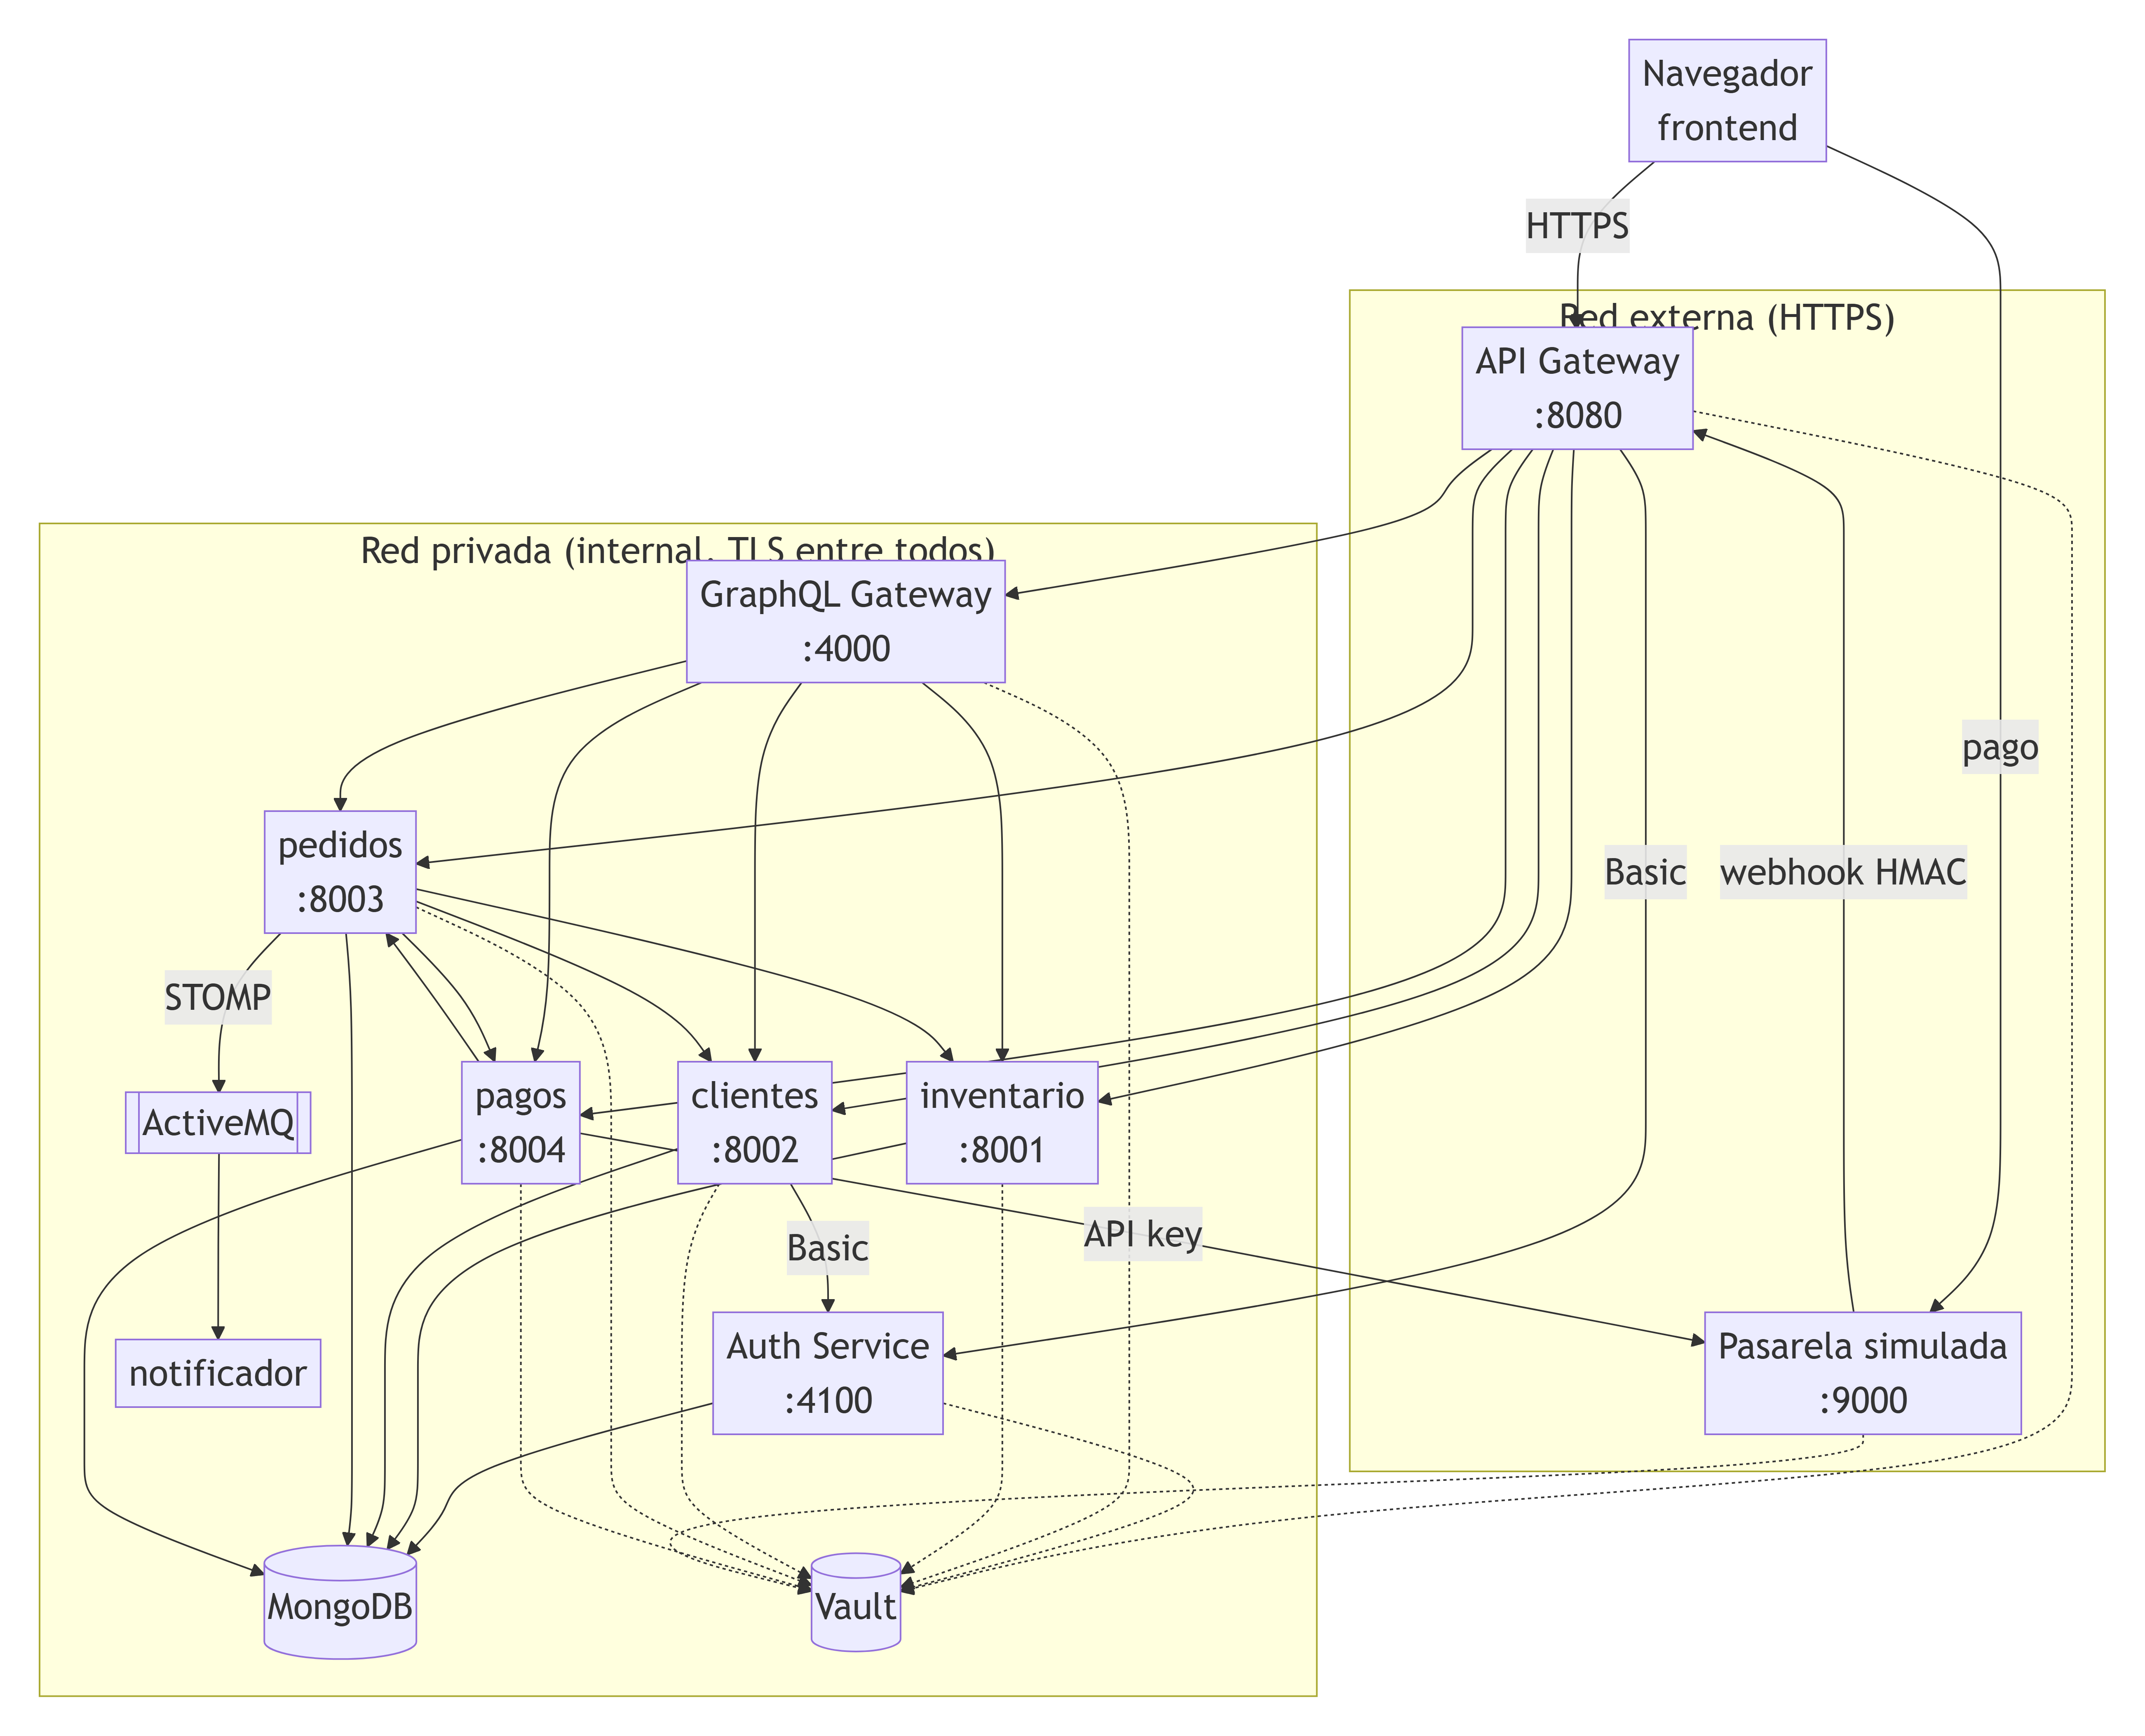
\includegraphics[width=\linewidth,height=0.85\textheight,keepaspectratio]{../diagramas/componentes.png}
\caption{Mapa de componentes}
\end{figure}

Leyenda: las flechas continuas son llamadas entre componentes (todas por TLS 1.2 o superior); \texttt{Basic} es HTTP Basic con un secreto de Vault, \texttt{API key} es la clave del comercio ante la pasarela y \texttt{webhook HMAC} es la notificación firmada; las líneas punteadas son la lectura de secretos en Vault, cada componente con su propio token; \texttt{STOMP} es la mensajería hacia ActiveMQ. El detalle de qué se verifica en cada salto está en la tabla de fronteras de confianza (sección 5).


Modelo C4 (\texttt{docs/\allowbreak{}diagramas/\allowbreak{}poke-\allowbreak{}fresh.\allowbreak{}dsl}): 25 vistas, validadas con el comando \texttt{validate} de Structurizr (imagen \texttt{structurizr/\allowbreak{}structurizr}) y exportables a Mermaid. Incluye C1 (contexto con la pasarela externa), C2 (contenedores, con recortes de catálogo, pedidos y pagos, y secretos), C3 de API Gateway, GraphQL Gateway, Auth Service y pedidos, vistas dinámicas de los flujos de los casos de validación (catálogo y su recuperación, pedido y su reintento, pedido propio y ajeno, sesión expirada, GraphQL con éxito, con error parcial y sobre el límite, pago, confirmación firmada y notificación falsa) y dos despliegues: \texttt{Docker\_\allowbreak{}Compose} (el entregado) y \texttt{Local\_\allowbreak{}Sin\_\allowbreak{}Docker} (pruebas, con Mongo, Vault y ActiveMQ en memoria). Para verlo: pegar el archivo en https://structurizr.com/dsl o usar el CLI. No hay imágenes renderizadas de estas vistas en el repositorio; los \texttt{.\allowbreak{}png} de arriba siguen siendo los diagramas de referencia del informe.


Despliegue (\texttt{docker-\allowbreak{}compose.\allowbreak{}yml}): 15 contenedores en dos redes (\texttt{tls-\allowbreak{}init}, \texttt{vault-\allowbreak{}init} y \texttt{semilla} son de un solo uso: crean los certificados, los secretos y los datos de ejemplo, respectivamente). \texttt{privada} es \texttt{internal:\allowbreak{} true} (sin puertos al equipo ni salida a Internet). Solo el gateway (8080) y la pasarela simulada (9000) publican puertos.


\begin{landscape}
\subsection{Secuencia de integración: compra completa}
\begin{figure}[H]
\centering
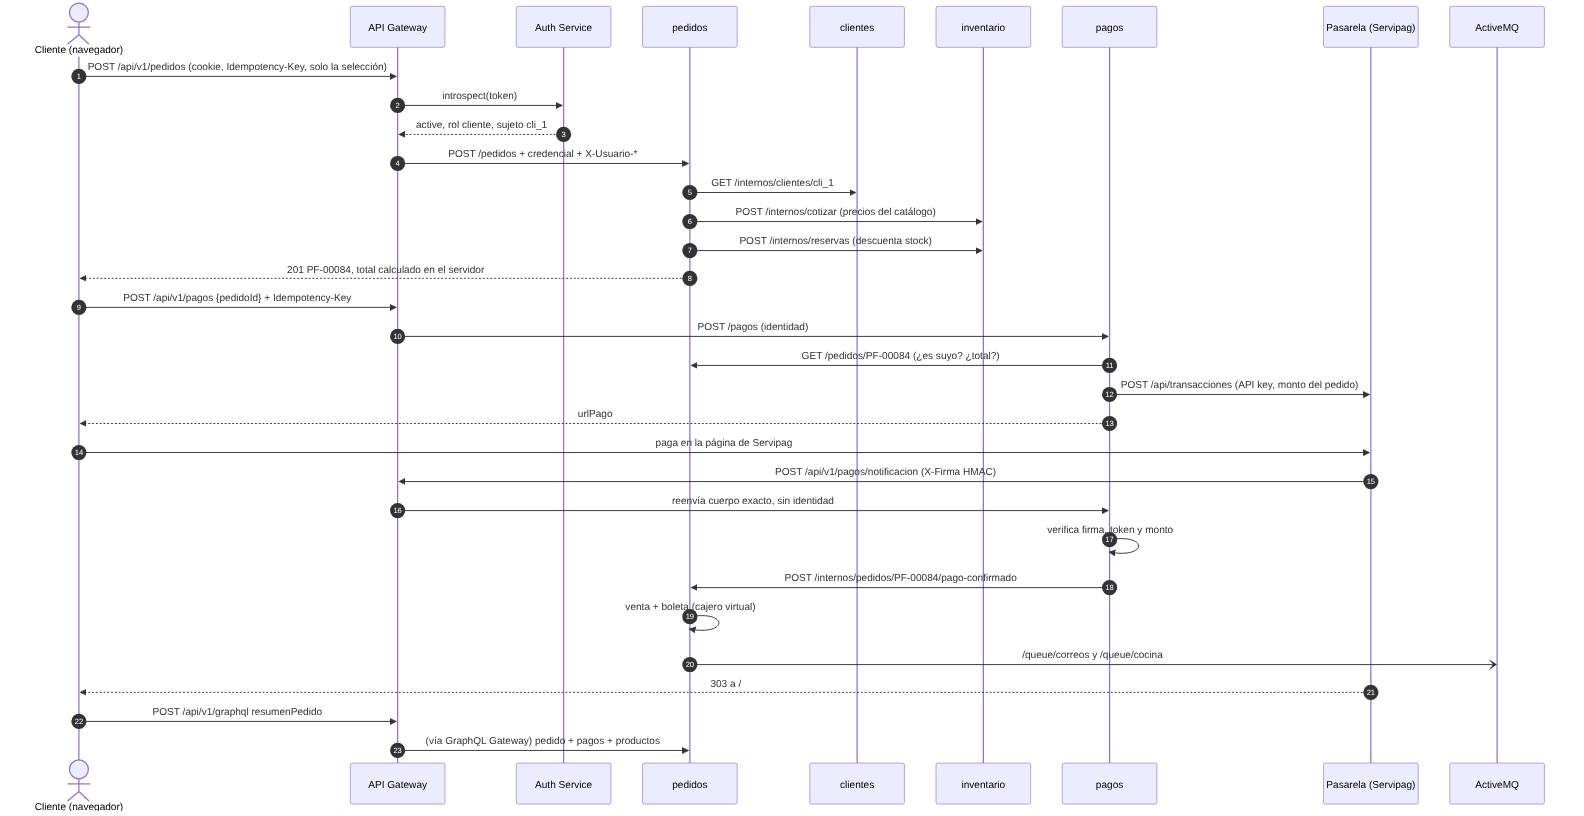
\includegraphics[width=\linewidth,height=0.78\textheight,keepaspectratio]{../diagramas/secuencia-compra.png}
\caption{Secuencia de compra}
\end{figure}
\end{landscape}

\subsection{Idempotencia del pago}

\begin{itemize}[nosep,leftmargin=*]
\item \textbf{Crear pedido:} \texttt{Idempotency-\allowbreak{}Key} opcional; el frontend genera una por visita a la pantalla de confirmación. Un doble clic devuelve el mismo pedido (índice único \texttt{idempotencia}).
\item \textbf{Iniciar pago:} \texttt{Idempotency-\allowbreak{}Key} obligatoria; misma clave $\rightarrow$ mismo pago. Si ya hay un pago pendiente para el pedido, se reutiliza.
\item \textbf{Notificación:} se aplica con una condición atómica (\texttt{estado:\allowbreak{} PENDIENTE} en el mismo \texttt{update}). Una repetida responde \texttt{repetido:\allowbreak{} true} sin volver a registrar la venta. Si pedidos no respondió la primera vez, la repetida reintenta solo ese aviso.
\item \textbf{Confirmación en pedidos:} si llega dos veces el mismo \texttt{pagoId}, la segunda no hace nada; el monto debe ser exactamente el total.
\item \textbf{Reservas de stock:} una por pedido; liberar dos veces devuelve el stock una sola vez.
\end{itemize}

Probado en \texttt{servicios/\allowbreak{}tests/\allowbreak{}test\_\allowbreak{}pedidos\_\allowbreak{}y\_\allowbreak{}pagos.\allowbreak{}py} y en los casos 10.2 y 10.3 de punta a punta.

